Now we discuss the training and test results of the A3C model that was described in Section~\ref{sec:a3c-method}. The asynchronous method of running the training means that we are unable to train on the GPU. This however means we are able to use all the available CPU cores by running 20 processes which each collects training information. This along with the reduced size of the input frames means the speed-up we get is significant. We are able to process $100$K frames in as little as 1 minute.

\medskip
\noindent
From the training graphs we see in Figure~\ref{fig:a3c-training} that irrespective of the rewards we use the model trains really fast and is able to converge withing the $80$M frames we trained all the networks for, which takes only a single day. We can see that in Figure~\ref{fig:training-a3c-05} that the rewards seem to make the model train in the first couple of million frames very well. To further analyze the training performance refer to Figure~\ref{fig:a3c-training-close}.


\begin{figure}[ht!]
    \centering
    \begin{subfigure}{0.49\textwidth}
        \centering
        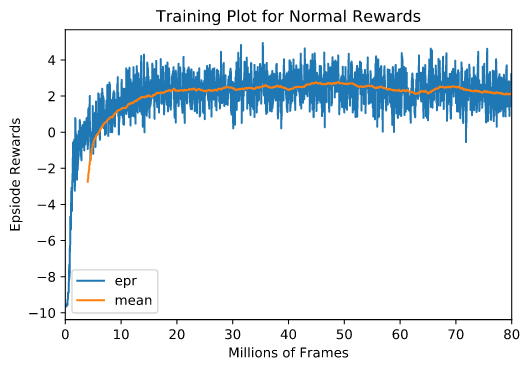
\includegraphics[width=\textwidth]{figures/a3c-training-normal.png}
        \caption{Normal Rewards}
        \label{fig:training-a3c-normal}
    \end{subfigure}
    \begin{subfigure}{0.49\textwidth}
        \centering
        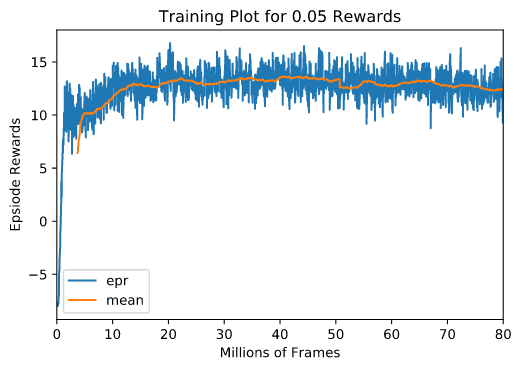
\includegraphics[width=\textwidth]{figures/a3c-training-0-05.png}
        \caption{Reward of $0.05$ for staying alive and $\pm 10$ at end}
        \label{fig:training-a3c-05}
    \end{subfigure}
    
    \begin{subfigure}{0.49\textwidth}
        \centering
        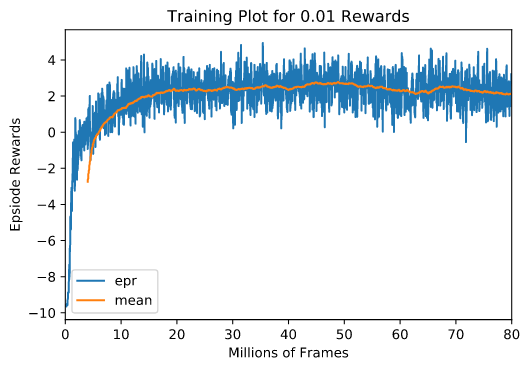
\includegraphics[width=\textwidth]{figures/a3c-training-0-01.png}
        \caption{Reward of $0.01$ for staying alive and $\pm 10$ at end}
        \label{fig:training-a3c-01}
    \end{subfigure}
    \caption{Training Graphs for a3C model with various rewards}
    \label{fig:a3c-training}
\end{figure}

Now looking at the first 10-12M frames in Figure~\ref{fig:a3c-training-close} we see the clear differences in the effect of the rewards used. There is one difference that has to be explained, is the range of the rewards that are from $-10$ to a varying range. This is because when providing a reward for staying alive, the model tends to stay alive in the 100s of timesteps, hence a reward of $0.01$ gives only $1$ accumulated compared to $5$ when it is $0.05$. Moving past this we see that the \textbf{normal rewards} takes longer to converge to a lower mean reward than the other two reward strategies, as see in Figure~\ref{fig:training-close-a3c-normal} and \ref{sub@fig:training-close-a3c-05}. We particularly see that for \textbf{0.05} rewards the learning rate is very fast reaching a mean reward of 10 by 2 million frames. 
\begin{figure}[ht!]
    \centering
    \begin{subfigure}{0.49\textwidth}
        \centering
        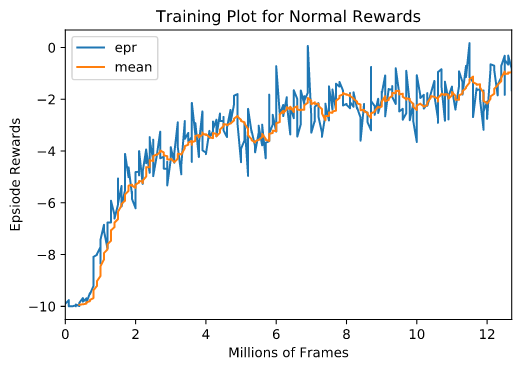
\includegraphics[width=\textwidth]{figures/a3c-training-normal_close.png}
        \caption{Normal Rewards}
        \label{fig:training-close-a3c-normal}
    \end{subfigure}
    \begin{subfigure}{0.49\textwidth}
        \centering
        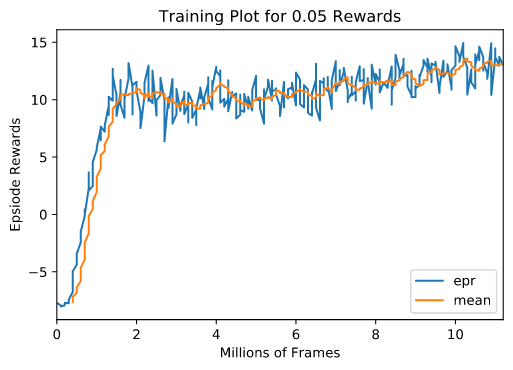
\includegraphics[width=\textwidth]{figures/a3c-training-0-05_close.png}
        \caption{Reward of $0.05$ for staying alive and $\pm 10$ at end}
        \label{fig:training-close-a3c-05}
    \end{subfigure}
    
    \begin{subfigure}{0.49\textwidth}
        \centering
        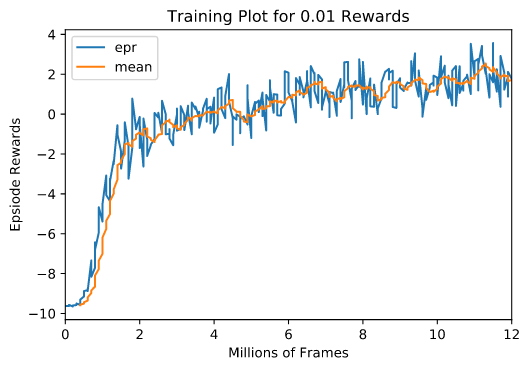
\includegraphics[width=\textwidth]{figures/a3c-training-0-01_close.png}
        \caption{Reward of $0.01$ for staying alive and $\pm 10$ at end}
        \label{fig:training-close-a3c-01}
    \end{subfigure}
    \caption{Closer look of training Graphs for a3C model with various rewards}
    \label{fig:a3c-training-close}
\end{figure}

Although training rewards are a good indicator of whether a model is training correctly or not, it is not necessarily an indicator of how well it will perform when tested against the SimpleAI which it trained against or other agents provided in the \texttt{test\_bench} code. We take the model saved at various stages of training till around 50 million frames and test it against 4 agents for 200 games. Due to the games being slightly random, this still provides a good estimate of the performance of the model. The results are seen in Figure~\ref{fig:a3c-testing}.

\medskip
\noindent
The most interesting results are those in Figure~\ref{fig:test-a3c-simpleai} which is the agent that we originally trained against. We see that there is some overfitting is happening as we move closer to 50 Million frames. To get a better idea we have Figure~\ref{fig-a3c-testing-simpleai-closer} where we look at the models till 20 million frames. We see that all the models start out at nearly 50\% win rate at 2 million frames. Then we see that the models that have rewards for staying alive, i.e. $0.01$ and $0.05$ rewards have better win rates. By 10 million frames the $0.01$ model achieves nearly 90\% win rate. We see in this time that the \textbf{normal rewards} are slower to converge to a better win rate, always behind the other 2 models. As we come to the 20 million mark zone we see this trend reversing, the $0.01$ and $0.05$ models start to overfit and the performance degrades to a win rate of high 80\% even see in Figure~\ref{sub@fig:test-a3c-simpleai}. After 20M frames the normal rewards model catches up and performs as well. This means that we need to stop training earlier for the other models.

\medskip
\noindent
From the perform against other agents we also see a similar trend, the normal rewards model takes longer to achieve the same performance but eventually by 50M frames outperforms the other models. This is clearly seen against \textit{SomeAgent} in Figure~\ref{sub@fig:test-a3c-someagent}. This confirms that the $0.01$ and $0.05$ rewards tend to overfit very soon. A thing to notice is that the model performs near optimally with 90\% win-rate against other models. This clearly indicates that the model has learnt to generalize well. 
\begin{figure}[th!]
    \centering
    \begin{subfigure}{0.49\textwidth}
        \centering
        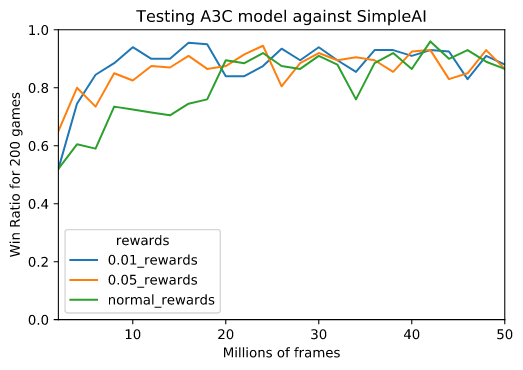
\includegraphics[width=\textwidth]{figures/a3c-test-simpleai.png}
        \caption{Against SimpleAI}
        \label{fig:test-a3c-simpleai}
    \end{subfigure}
    \begin{subfigure}{0.49\textwidth}
        \centering
        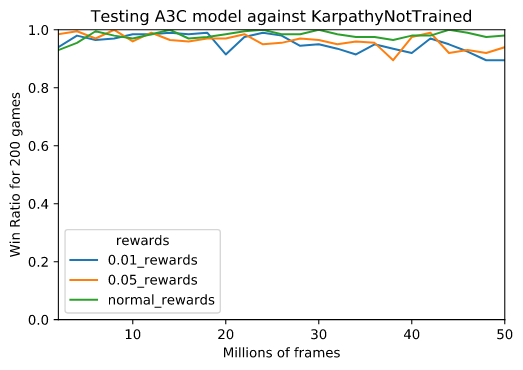
\includegraphics[width=\textwidth]{figures/a3c-test-karpathy-not-trained.png}
        \caption{Against KarpathyNotTrained}
        \label{fig:test-a3c-karpathy}
    \end{subfigure}

    \begin{subfigure}{0.49\textwidth}
        \centering
        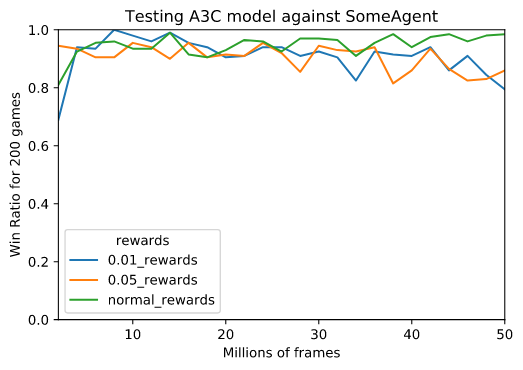
\includegraphics[width=\textwidth]{figures/a3c-test-someagent.png}
        \caption{Against SomeAgent}
        \label{fig:test-a3c-someagent}
    \end{subfigure}
    \begin{subfigure}{0.49\textwidth}
        \centering
        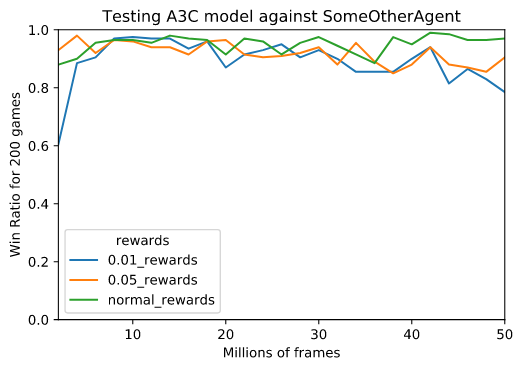
\includegraphics[width=\textwidth]{figures/a3c-test-someaothergent.png}
        \caption{Against SomeOtherAgent}
        \label{fig:test-a3c-someotheragent}
    \end{subfigure}
    
    \caption{Test of A3C model against agents}
    \label{fig:a3c-testing}
\end{figure}

\begin{figure}[ht!]
    \centering
    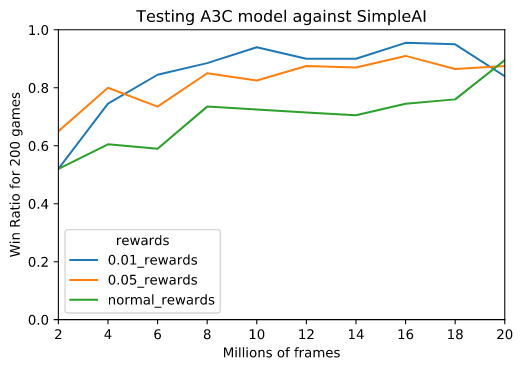
\includegraphics[width=0.5\textwidth]{figures/a3c-test-simpleai-close.png}
    \caption{Closer look at SimpleAI test results}
    \label{fig-a3c-testing-simpleai-closer}
\end{figure}